\documentclass{article}
\usepackage{pgfplots} 
\title{Homework 2 \\
	\large Encryption / decryption comparison}
\author{Fabio Massimo Ercoli
	\footnote{
		More on me:
		https://github.com/fax4ever
		https://www.linkedin.com/in/fabioercoli/
}}
\date{October 20\textsuperscript{st} 2024}
\pgfplotsset{compat=1.8} 

\begin{document}
	
\maketitle
\thispagestyle{empty}

\section{Compile and run the algorithms}

\subsection{Source code content}

The zip file named \textbf{symmetric-encryption.zip} contains the source code:
\begin{itemize}
	\item \textbf{aes-cbc.c}: AES 128 CBC encryption / decryption
	\item \textbf{aria-cbc.c}: ARIA 128 CBC encryption / decryption
	\item \textbf{camellia-cbc.c}: Camellia 128 CBC encryption / decryption
	\item \textbf{aes-cbc.c}: AES 128 CBF encryption / decryption (I tried a different operation mode also)
\end{itemize}

and the files to encrypt / decrypt:

\begin{itemize}
	\item \textbf{1k.txt}: 1 kB text file
	\item \textbf{10.txt}: 10 kB text file
	\item \textbf{large-binary.MP4}: > 1MB binary file
\end{itemize}

\subsection{Compille the code}

I downloaded, compiled and installed the OpenSSL 3.3.2 libraries under the local directory of my Fedora Linux file system:
\begin{verbatim}
	/home/fax/lib/openssl-3.3.2/
\end{verbatim}	

To compile my files I run the commands in any order:

\begin{verbatim}
	gcc aes-cbc.c -o aes-cbc -I /home/fax/lib/openssl-3.3.2/include \
	-L /home/fax/lib/openssl-3.3.2/lib64 -lcrypto
\end{verbatim}

\begin{verbatim}
	gcc aria-cbc.c -o aria -I /home/fax/lib/openssl-3.3.2/include \
	-L /home/fax/lib/openssl-3.3.2/lib64 -lcrypto
\end{verbatim}	

\begin{verbatim}
	gcc camellia-cbc.c -o camellia -I /home/fax/lib/openssl-3.3.2/include \
	-L /home/fax/lib/openssl-3.3.2/lib64 -lcrypto
\end{verbatim}	

\begin{verbatim}
	gcc aes-cbf.c -o aes-cbf -I /home/fax/lib/openssl-3.3.2/include \
	-L /home/fax/lib/openssl-3.3.2/lib64 -lcrypto
\end{verbatim}

\subsection{Encrypt / decrypt the test files}		

\begin{itemize}
	\item run \textbf{./aes-cbc}  to encrypt / decrypt the files using  AES 128 CBC
	\item run \textbf{./aria-cbc}  to encrypt / decrypt the files using  Aria 128 CBC
	\item run \textbf{./camellia-cbc}  to encrypt / decrypt the files using  Camellia 128 CBC
	\item run \textbf{./aes-cbf}  to encrypt / decrypt the files using  AES 128 CBF
\end{itemize}

After running those commands more files are generated. In particular one file as a result of the decryption and one file as the result of the encryption for each original file and for each algorithm.

For instance \emph{large-binary-ari.dat} is the result of the encryption using Aria 128 CBC of the original binary file \emph{large-binary-ari.MP4}. While \emph{large-binary-ari-dec.MP4} is the result of the decryption using Aria 128 CBC of the encrypted binary file \emph{large-binary-ari.dat}. 

In our implementation \emph{large-binary-ari-dec.MP4} must be identical to the original one \emph{large-binary-ari.dat}.

And this must be true for all the combinations of files / algorithms.

You can check the file names looking at the console output logs.

\subsection{Console output for execution}

Here is an execution.
You can notice that both the secret keys and the initialization vectors are randomly generated, in particular using a random generation API of Open SSL.

\begin{verbatim}
fax@fedora:~/Documents/study-more/cyber/homeworks/h2/symmetric-encryption$ ./aria 

The key : 27 C1 F8 E0 E8 BE 7D 16 75 6C 50 E0 66 3C 92 D3 
The IV  : 82 58 8A 70 2B D9 92 17 7C 11 9F 4F 2F 84 1A BC 
Aria CBC << encrypt >> 1k.txt -> 1k-ari.dat:		 24 microseconds
Aria CBC << decript >> 1k-ari.dat -> 1k-ari-dec.txt:		 15 microseconds
Aria CBC << encrypt >> 10k.txt -> 10k-ari.dat:		 76 microseconds
Aria CBC << decript >> 10k-ari.dat -> 10k-ari-dec.txt:		 60 microseconds
Aria CBC << encrypt >> large-binary.MP4 -> large-binary-ari.dat:		 21248 microseconds
Aria CBC << decript >> large-binary-ari.dat -> large-binary-ari-dec.MP4:		 18136 microseconds

fax@fedora:~/Documents/study-more/cyber/homeworks/h2/symmetric-encryption$ ./aes-cbc 

The key : 10 48 8A A3 FB AB FA 75 D4 28 0C 7D 4B 24 D7 AC 
The IV  : CB 5F 5F 92 C6 AE 9B 4A AD 32 B3 13 32 9C C2 7C 
AES CBC << encrypt >> 1k.txt -> 1k-cbc.dat:		 12 microseconds
AES CBC << decrypt >> 1k-cbc.dat -> 1k-cbc-dec.txt:		 9 microseconds
AES CBC << encrypt >> 10k.txt -> 10k-cbc.dat:		 59 microseconds
AES CBC << decrypt >> 10k-cbc.dat -> 10k-cbc-dec.txt:		 90 microseconds
AES CBC << encrypt >> large-binary.MP4 -> large-binary-cbc.dat:		 19761 microseconds
AES CBC << decrypt >> large-binary-cbc.dat -> large-binary-cbc-dec.MP4:		 25073 microseconds

fax@fedora:~/Documents/study-more/cyber/homeworks/h2/symmetric-encryption$ ./camellia 

The key : C3 A8 9D AB A4 C2 B2 E7 A9 DF 09 31 0D 6F 84 B2 
The IV  : 09 21 C9 52 45 24 E3 7B 38 74 F6 95 F6 AD FB 17 
Camellia CBC << encrypt >> 1k.txt -> 1k-cam.dat:		 12 microseconds
Camellia CBC << decrypt >> 1k-cam.dat -> 1k-cam-dec.txt:		 5 microseconds
Camellia CBC << encrypt >> 10k.txt -> 10k-cam.dat:		 54 microseconds
Camellia CBC << decrypt >> 10k-cam.dat -> 10k-cam-dec.txt:		 45 microseconds
Camellia CBC << encrypt >> large-binary.MP4 -> large-binary-cam.dat:		 16318 microseconds
Camellia CBC << decrypt >> large-binary-cam.dat -> large-binary-cam-dec.MP4:		 13364 microseconds

fax@fedora:~/Documents/study-more/cyber/homeworks/h2/symmetric-encryption$ ./aes-cbf

The key : 8E F5 78 EA 20 F0 B3 E8 DA 62 FE CF C6 D2 2E B5 
The IV  : 40 22 E0 DF 01 06 04 63 B8 6D 06 E2 D0 89 9A D1 
AES CFB 128 << encrypt >> 1k.txt -> 1k-aes.dat:		 14 microseconds
AES CFB 128 << decrypt >> 1k-aes.dat -> 1k-aes-dec.txt:		 7 microseconds
AES CFB 128 << encrypt >> 10k.txt -> 10k-aes.dat:		 67 microseconds
AES CFB 128 << decrypt >> 10k-aes.dat -> 10k-aes-dec.txt:		 68 microseconds
AES CFB 128 << encrypt >> large-binary.MP4 -> large-binary-aes.dat:		 25146 microseconds
AES CFB 128 << decrypt >> large-binary-aes.dat -> large-binary-aes-dec.MP4:		 24757 microseconds	
\end{verbatim}	

\section{Collect the results}

We have 6 values collected for each algorithms (that are the encryption and the decryption of each test file).

Averaging the result of three distinct executions, I got the following results:

\begin{tabular}{ c c c c c }
	Microseconds & AES CBC & ARIA CBC  &CAMELLIA CBC & AES CBF  \\
	1K  encrypt  & 15.7 & 23.7 & 11 & 14.3 \\
	1K decrypt & 9 & 17 & 5.3 & 8 \\
	10K  encrypt  & 58 & 70.3 & 54.3 & 69.7 \\
	10K  decrypt  &75 & 62 & 41 & 72 \\
	1M+  encrypt  & 19000 & 21176 & 16079.7 & 22537.3 \\
	1M+  decrypt  & 25095.3 & 18003.3 & 13170.3 & 22838.7 \\
\end{tabular}

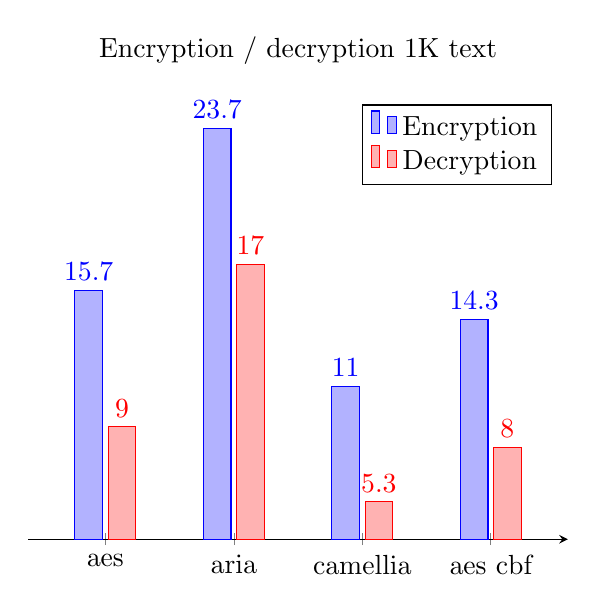
\begin{tikzpicture}
	\begin{axis}[ybar, title={Encryption / decryption 1K text}, symbolic x coords={aes, aria, camellia, aes cbf},
		legend pos = north east, axis y line=none, axis x line=bottom, nodes near coords, enlarge x limits=0.2, ] 
		\addplot+ coordinates {(aes, 15.7) (aria, 23.7) (camellia, 11) (aes cbf, 14.3)}; 
		\addplot+ coordinates {(aes, 9) (aria, 17) (camellia, 5.3) (aes cbf, 8)};
		\legend{Encryption, Decryption}; \end{axis} 
\end{tikzpicture} 

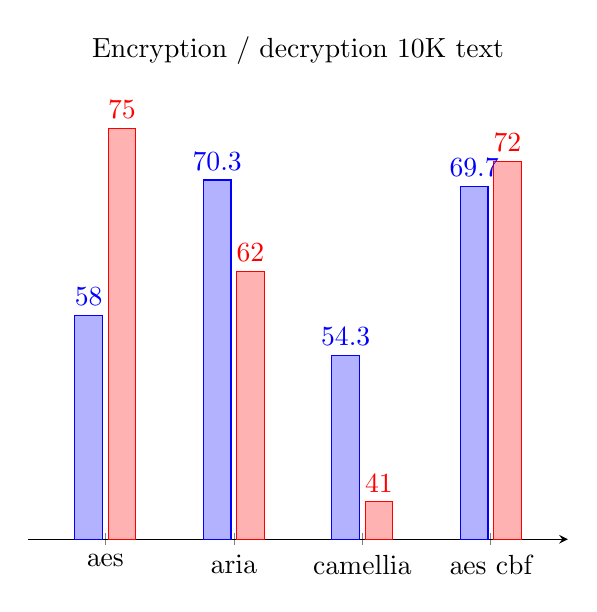
\begin{tikzpicture}
	\begin{axis}[ybar, title={Encryption / decryption 10K text}, symbolic x coords={aes, aria, camellia, aes cbf},
		legend pos = north east, axis y line=none, axis x line=bottom, nodes near coords, enlarge x limits=0.2, ] 
		\addplot+ coordinates {(aes, 58) (aria, 70.3) (camellia, 54.3) (aes cbf, 69.7)}; 
		\addplot+ coordinates {(aes, 75) (aria, 62) (camellia, 41) (aes cbf, 72)};
		\end{axis} 
\end{tikzpicture}

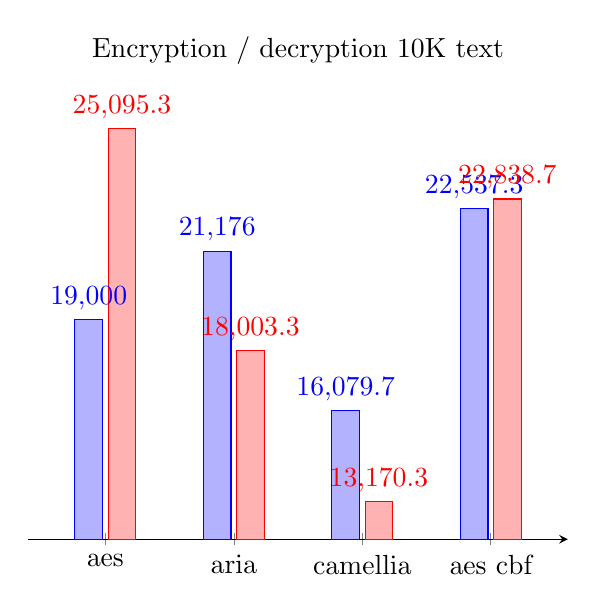
\begin{tikzpicture}
	\begin{axis}[ybar, title={Encryption / decryption 10K text}, symbolic x coords={aes, aria, camellia, aes cbf},
		legend pos = north east, axis y line=none, axis x line=bottom, nodes near coords, enlarge x limits=0.2, ] 
		\addplot+ coordinates {(aes, 19000) (aria, 21176) (camellia, 16079.7) (aes cbf, 22537.3)}; 
		\addplot+ coordinates {(aes, 25095.3) (aria, 18003.3) (camellia, 13170.3) (aes cbf, 22838.7)};
	\end{axis} 
\end{tikzpicture}

\end{document}	